\chapter{ЛИТЕРАТУРНЫЙ ОБЗОР}
\section{Введение}
Аппарат для тренировки и контроля аккомодации является простым прибором. При работе пациент наблюдает через монокулярную оптическую систему тест-объект. За счет его перемещения изменяется положение наблюдаемого изображения относительно глаза пациента. Разные тест-объекты, ориентированны на функционально различное назначение. 

Фиксируя крайние положения резко наблюдаемого объекта, можно проконтролировать аметропию  для дали и для близи, а также объем аккомодации. Плавное перемещение объекта в пределах объема аккомодации обеспечивает возможность тренировки механизма аккомодации глаза. Острота зрения для дали и для близи контролируется при использовании тест-объектов с таблицами различных оптотипов.

Аккомодометр позволяет исследовать астигматизм и определять главные меридианы астигматического глаза. Проводить контроль ночной миопии при пониженной яркости или освещенности тест-объекта. 

Все измерения осуществляются субъективным методом, поскольку основаны на оценке пациентом качества наблюдаемого изображения.

Аппарат рекомендуется для использования в офтальмологической практике при лечебных и оздоровительных мероприятиях. По назначению лечащего врача-офтальмолога аппарат может использоваться в домашних условиях, как правило, для проведения процедур по тренировке аккомодации, закрепляющих амбулаторное лечение. Длительность и периодичность воздействия устанавливаются в зависимости от медицинских показаний.

\section{Устройство и принцип действия}
Аппарат может использоваться для контроля объема аккомодации (как проксиметр), а также для определения аметропии, астигматизма и направления главных меридианов астигматического глаза (как оптиметр). 

Действие аппарата основано на монокулярном наблюдении слайда(или картинки дисплея), изображение которого может перемещаться относительно глаза пациента. На рис.\ref{fig:OpticSche} изображена оптическая схема аппарата. Наблюдаемым тест-обьектом может быть как дисплей 5 или освещенный дисплеем слайд 6.

\begin{figure}[ht]
	\centering
     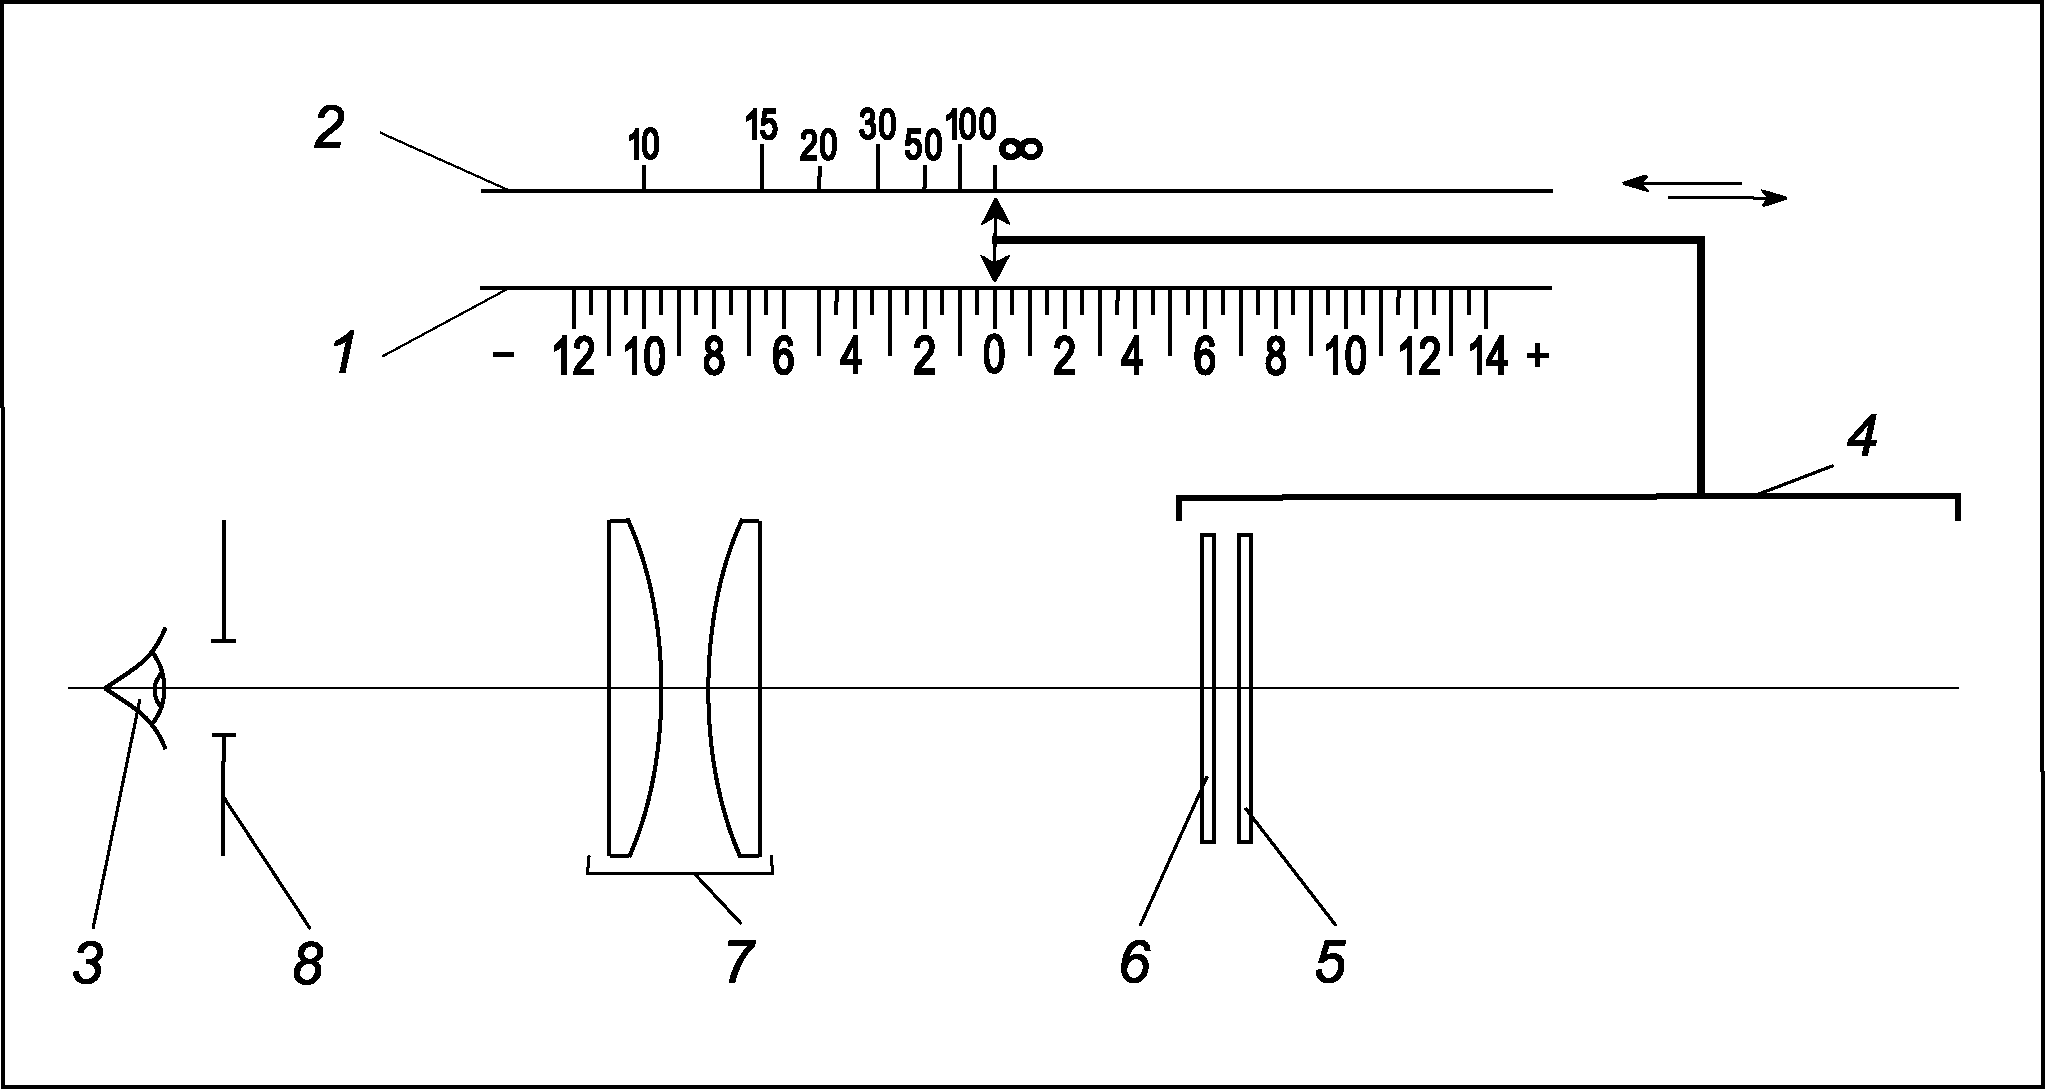
\includegraphics[scale=0.7]{The_optical_scheme_of_the_device.png}
	\caption{Оптическая схема аппарата.}
	\label{fig:OpticSche}
\end{figure}

При использовании слайда, между экраном и слайдом помещается матовый светофильтр. Объектив 7 формирует изображение объекта. Это изображение наблюдается глазом 3, который располагается вблизи выходного зрачка 8 оптической системы. Компоненты 5 и 6 конструктивно образуют узел каретки 4, перемещаемый относительно остальной части оптической системы. 

Положение каретки контролируется по шкалам 1 и 2. Верхняя шкала 2 оцифрованным в сантиметрах и определяет расстояние $S$ между изображением и глазом. Если объект располагается в фокусе объектива (как это показано на рис. \ref{fig:OpticSche}), то изображение находится в бесконечности($ S=\infty $). При перемещении объекта влево (ближе к глазу) объектив формирует мнимое изображение, когда точка пересечения лучей, прошедших через объектив, находится правее объектива. Расстояние $S$ изменяется от максимального значения (свыше $100$ см) до минимальной величины (менее $10$ см).

Нижняя шкала 1 оцифрована в диоптриях и предназначена для определения аметропии глаза (А). Показания шкал связаны между собой соотношением $ A=\frac{-100}{S}$. Расположение объекта в фокусе  ($ S=\infty $) соответствует нулевому отсчету по диоптрийной шкале: $A=0$.

Чем ближе каретка к глазу, тем на меньшем расстоянии наблюдается изображение. Так, например, при $A=-2$ дптр изображение находится от глаза на расстоянии $S=50$ см, при $A =-4$ дптр на расстоянии $25$ см.
Положительные значения аметропии соответствуют смещению объекта правее фокуса. При этом объектив формирует действительное изображение, расположенное левее глаза.

\section{Режимы работы}
\subsection{Контроль аметропии}
Аметропия определяется в двух точках в ближней и дальней, максимальная острота зрения соответствует моменту, когда главный фокус глаза располагается на сетчатке, а значит это положение, если оно крайнее, дальняя или ближняя точка. Ниже на рис.\ref{fig:TestObjC} приведено изображение используемое для тест-объектов.

\begin{figure}[ht]
	\centering
	
\includegraphics[scale=1]{Test_Obj_Cycles.png}
	\caption{Расположение знаков в тест-объекте.}
	\label{fig:TestObjC}
\end{figure}
\subsection{Контроль объема аккомодации}
Объем аккомодации($\triangle A$ см. табл.\ref{tab:AccDuane}) это то расстояние между ближней и дальней точкой, в которой глаз четко видит изображение. Следовательно его определения определяются ближняя и дальняя точка, и находится их разность.
\begin{table}
\centering
\begin{tabular}{|c|c|c|c|}
\hline 
Возраст, лет &$\triangle A$,дптр & Возраст, лет & $\triangle A$,дптр \\ 
\hline 
10 & 12 - 14 & 40 & 3 - 8 \\ 
\hline 
16 & 10 - 14 & 45 & 2 - 6 \\ 
\hline 
20 & 9 - 13 & 50 & 1 – 3 \\ 
\hline 
25 & 8 - 12 & 55 & 0,75 – 1,75 \\ 
\hline 
30 & 6 - 10 & 60 & 0,5 – 1,5 \\ 
\hline 
35 & 5 - 9 & • & • \\ 
\hline 
\end{tabular} 
\caption{Возрастные нормы абсолютной аккомодации (по Дуане).}
\label{tab:AccDuane}
\end{table}
\subsection{Проведение тренировки аккомодации}
Тренировка механизма аккомодации глаза производится при перемещении слайда в пределах установленного объема аккомодации с периодическими попытками расширения его границ. Тренировку проводят поочередно каждым глазом.При тренировке плавно перемещают слайд от дальней границы резкого видения к ближней границе и обратно. Следует стремиться к расширению границ аккомодации: при близорукости – дальней границы, при дальнозоркости – ближней. Приближение слайда к границе аккомодации будет приводить к размытию изображения.  Продолжительности тренировки каждого глаза составляет 3 ... 7 мин. В профилактических целях тренировку можно проводить после работы, связанной со значительными зрительными нагрузками.
\subsection{Контроль остроты зрения}
Контроль остроты зрения проводится с помощью специальных слайдов см. рис.\ref{fig:TestObjEC}. Особенности построения оптической системы аппарата обеспечивают сохранение углового размера знака при перемещении слайда. За счет этого один и тот же слайд может использоваться для контроля зрения вдаль и вблизи.

\begin{figure}[ht]
    \centering
    \begin{subfigure}[b]{0.3\textwidth}
    \centering
        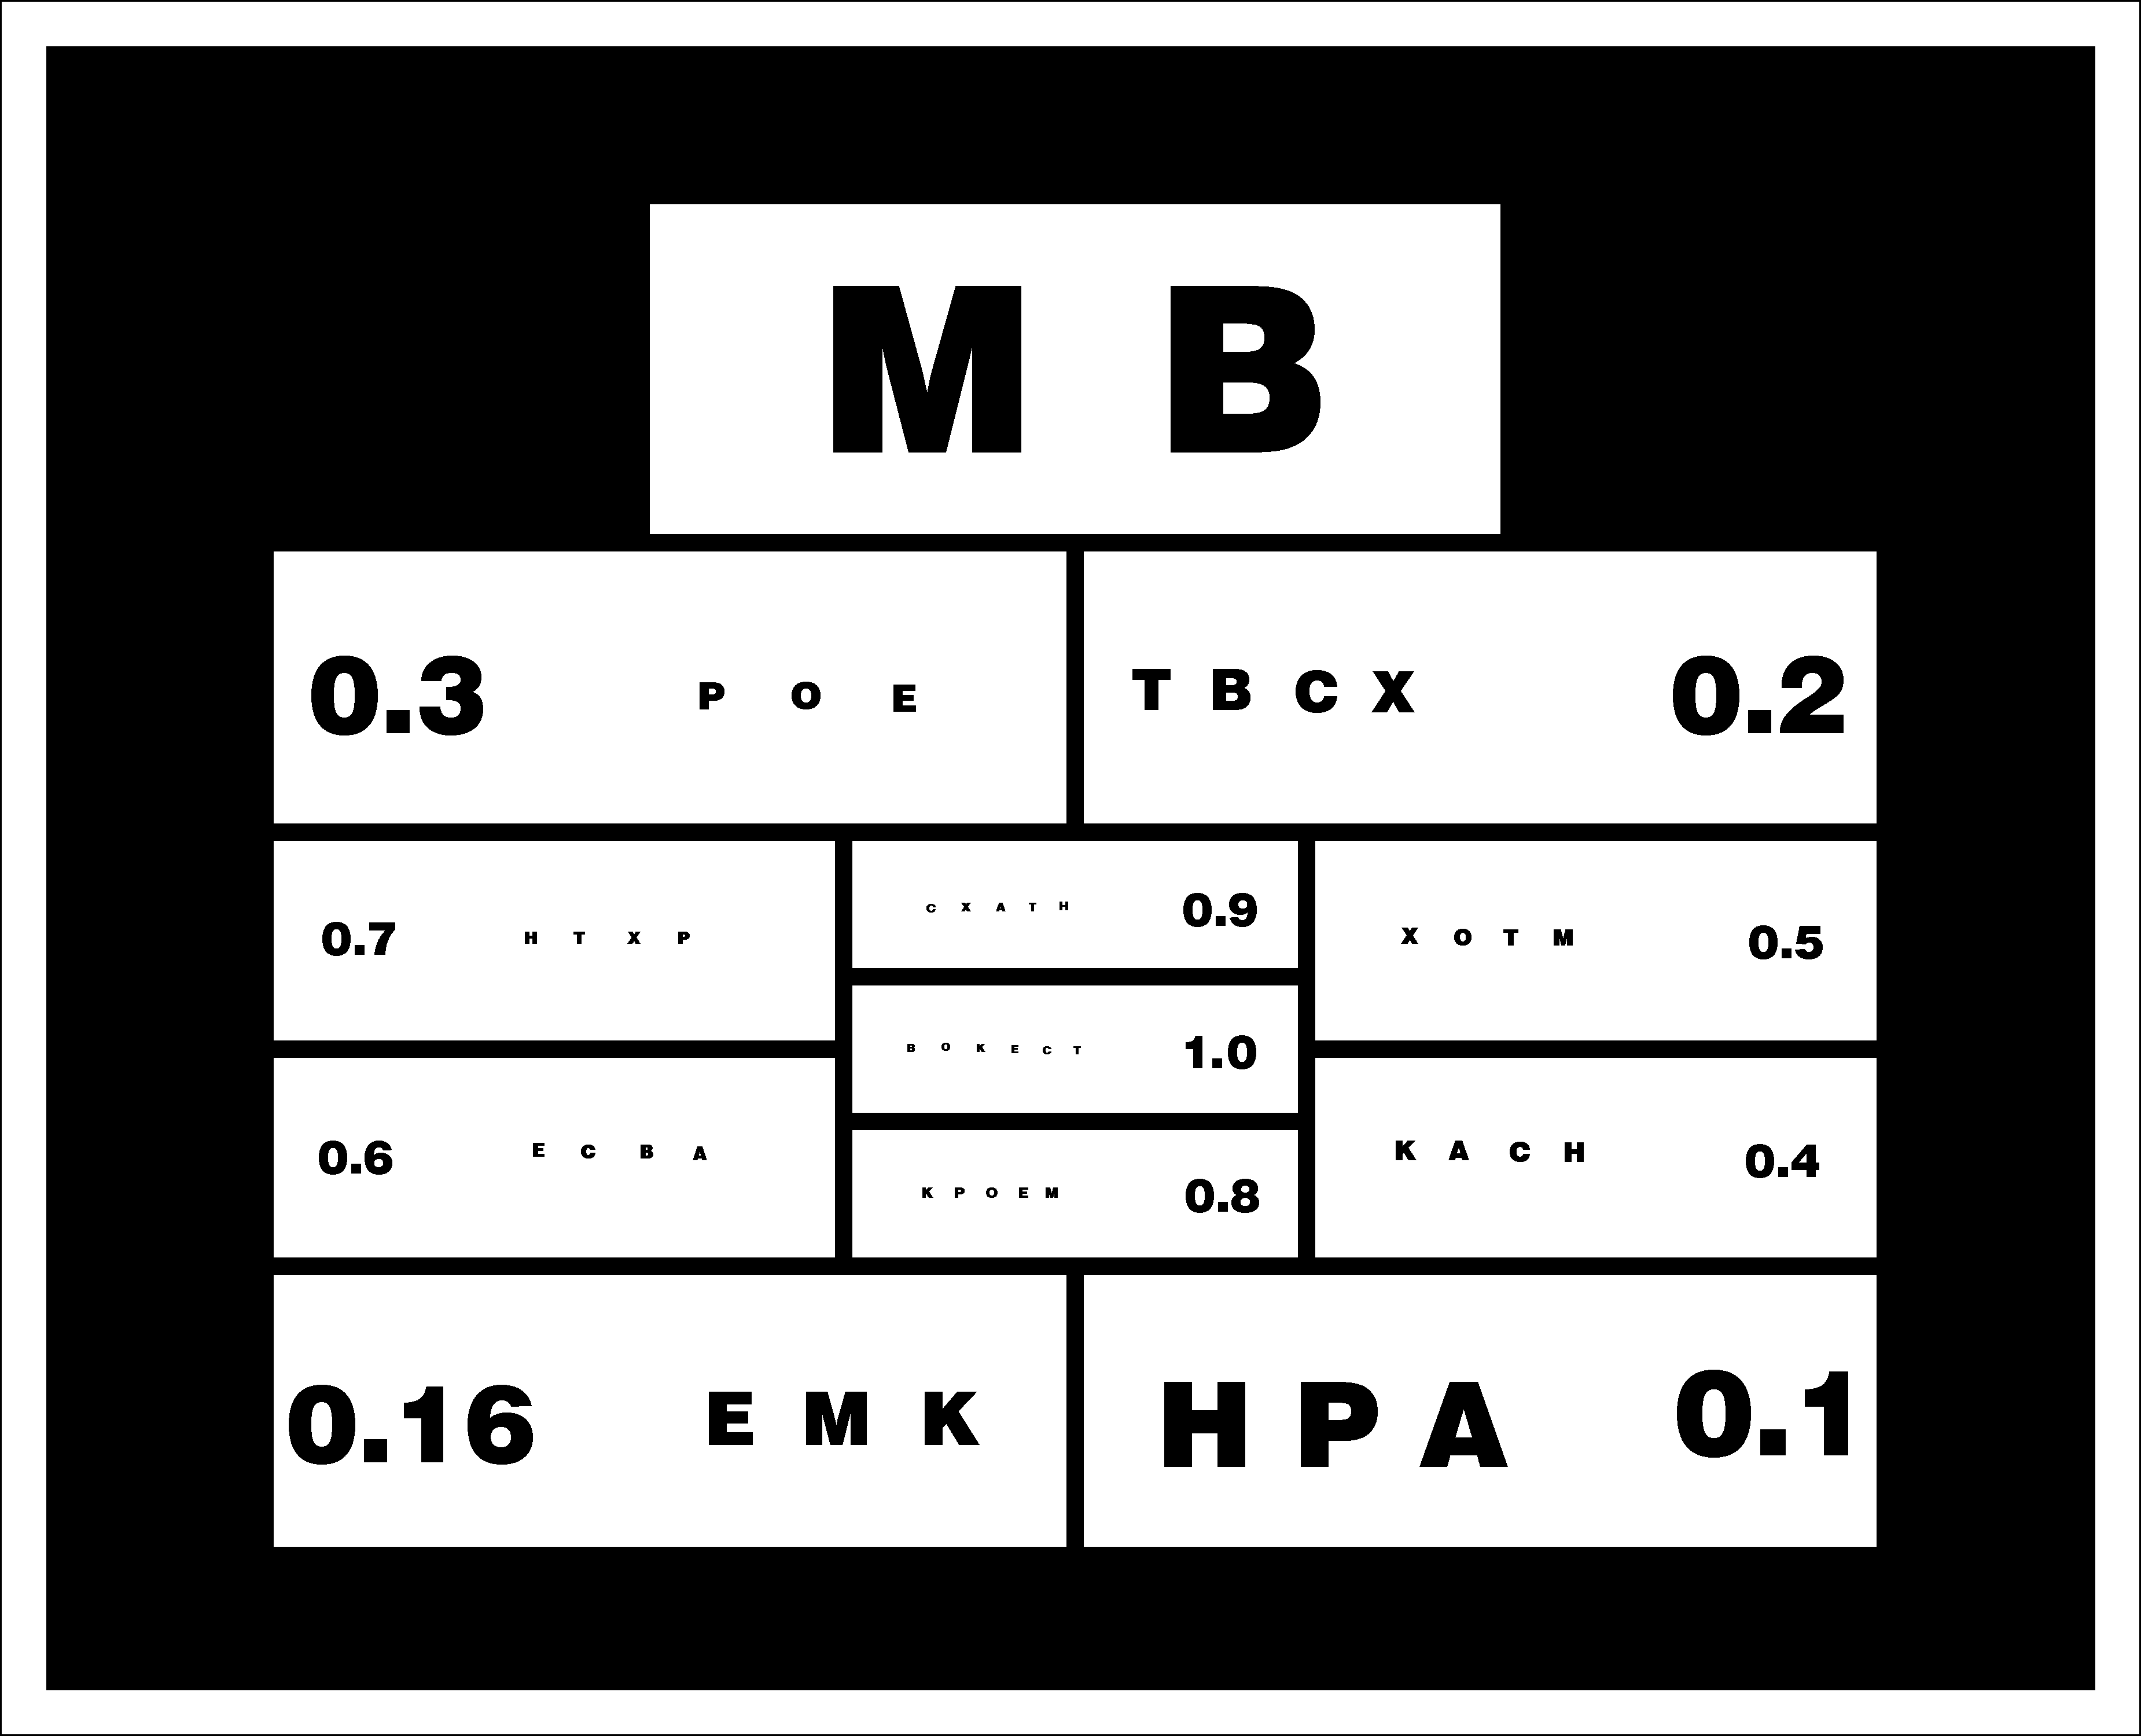
\includegraphics[scale=2]{Test_Obj_eye_control1.png}
        \caption{}
    \end{subfigure}
    \begin{subfigure}[b]{0.3\textwidth}
    \centering
        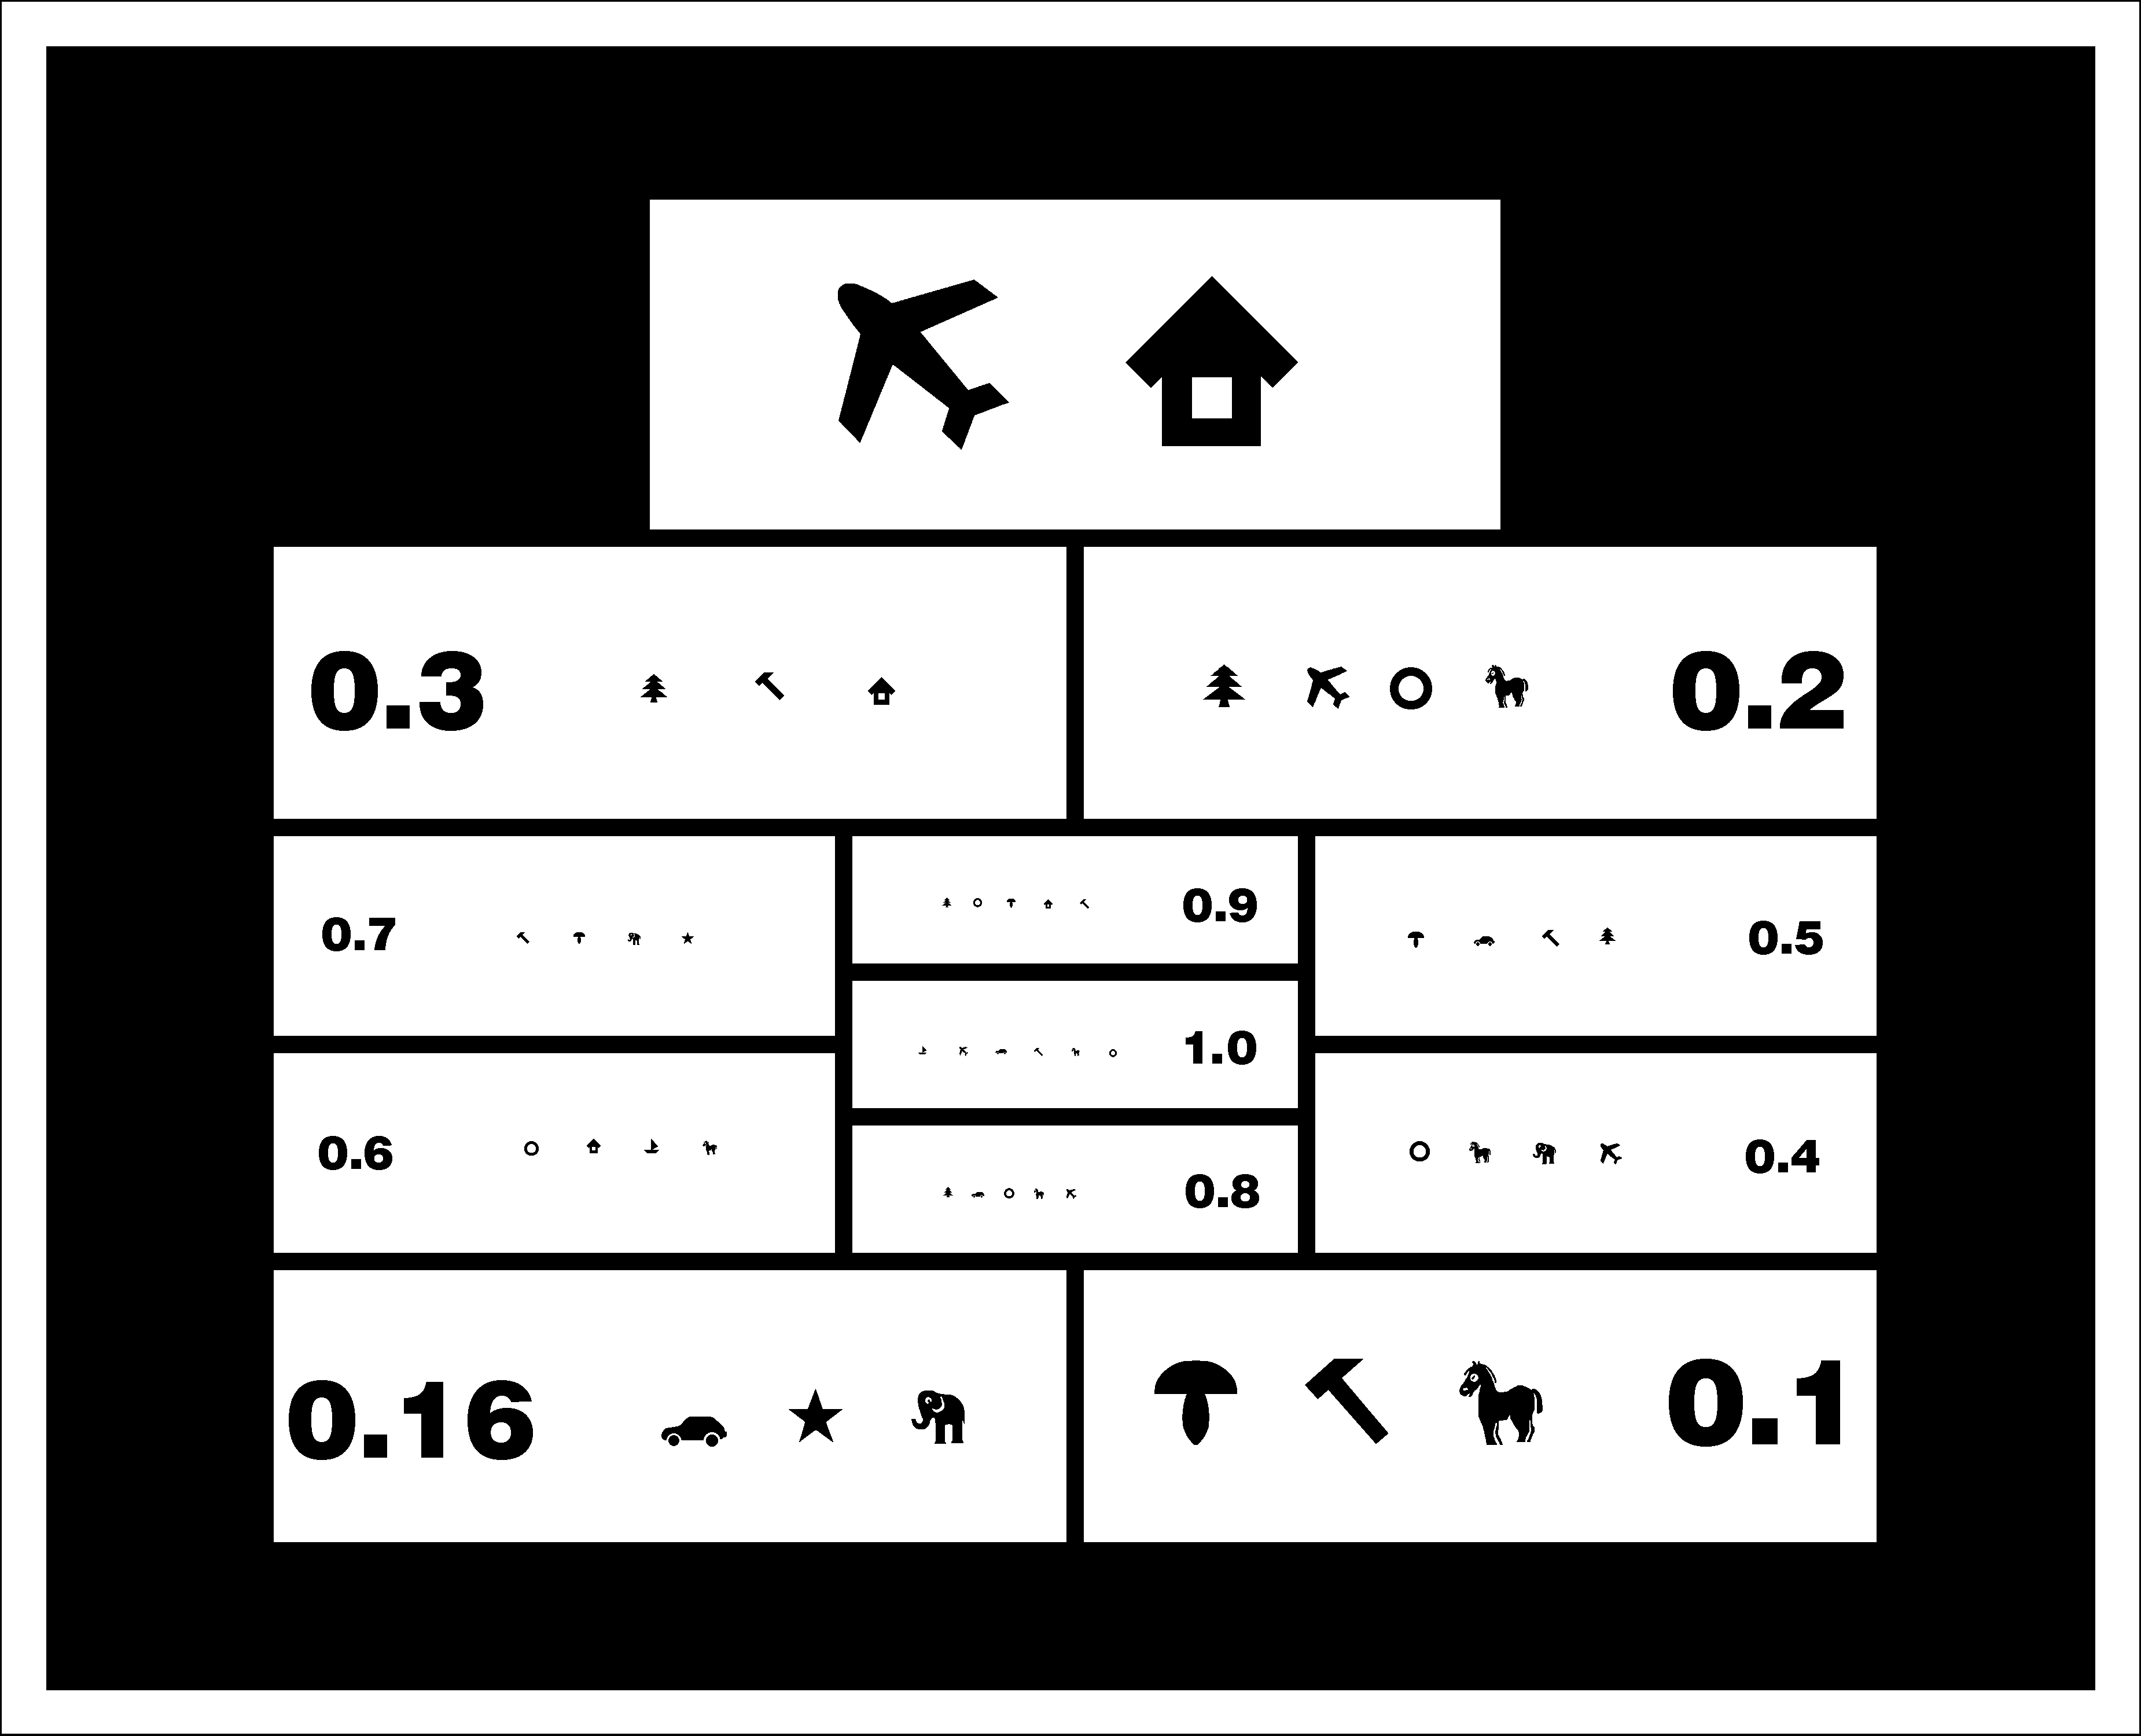
\includegraphics[scale=2]{Test_Obj_eye_control2.png}
        \caption{}
    \end{subfigure}
    \begin{subfigure}[b]{0.3\textwidth}
    \centering
        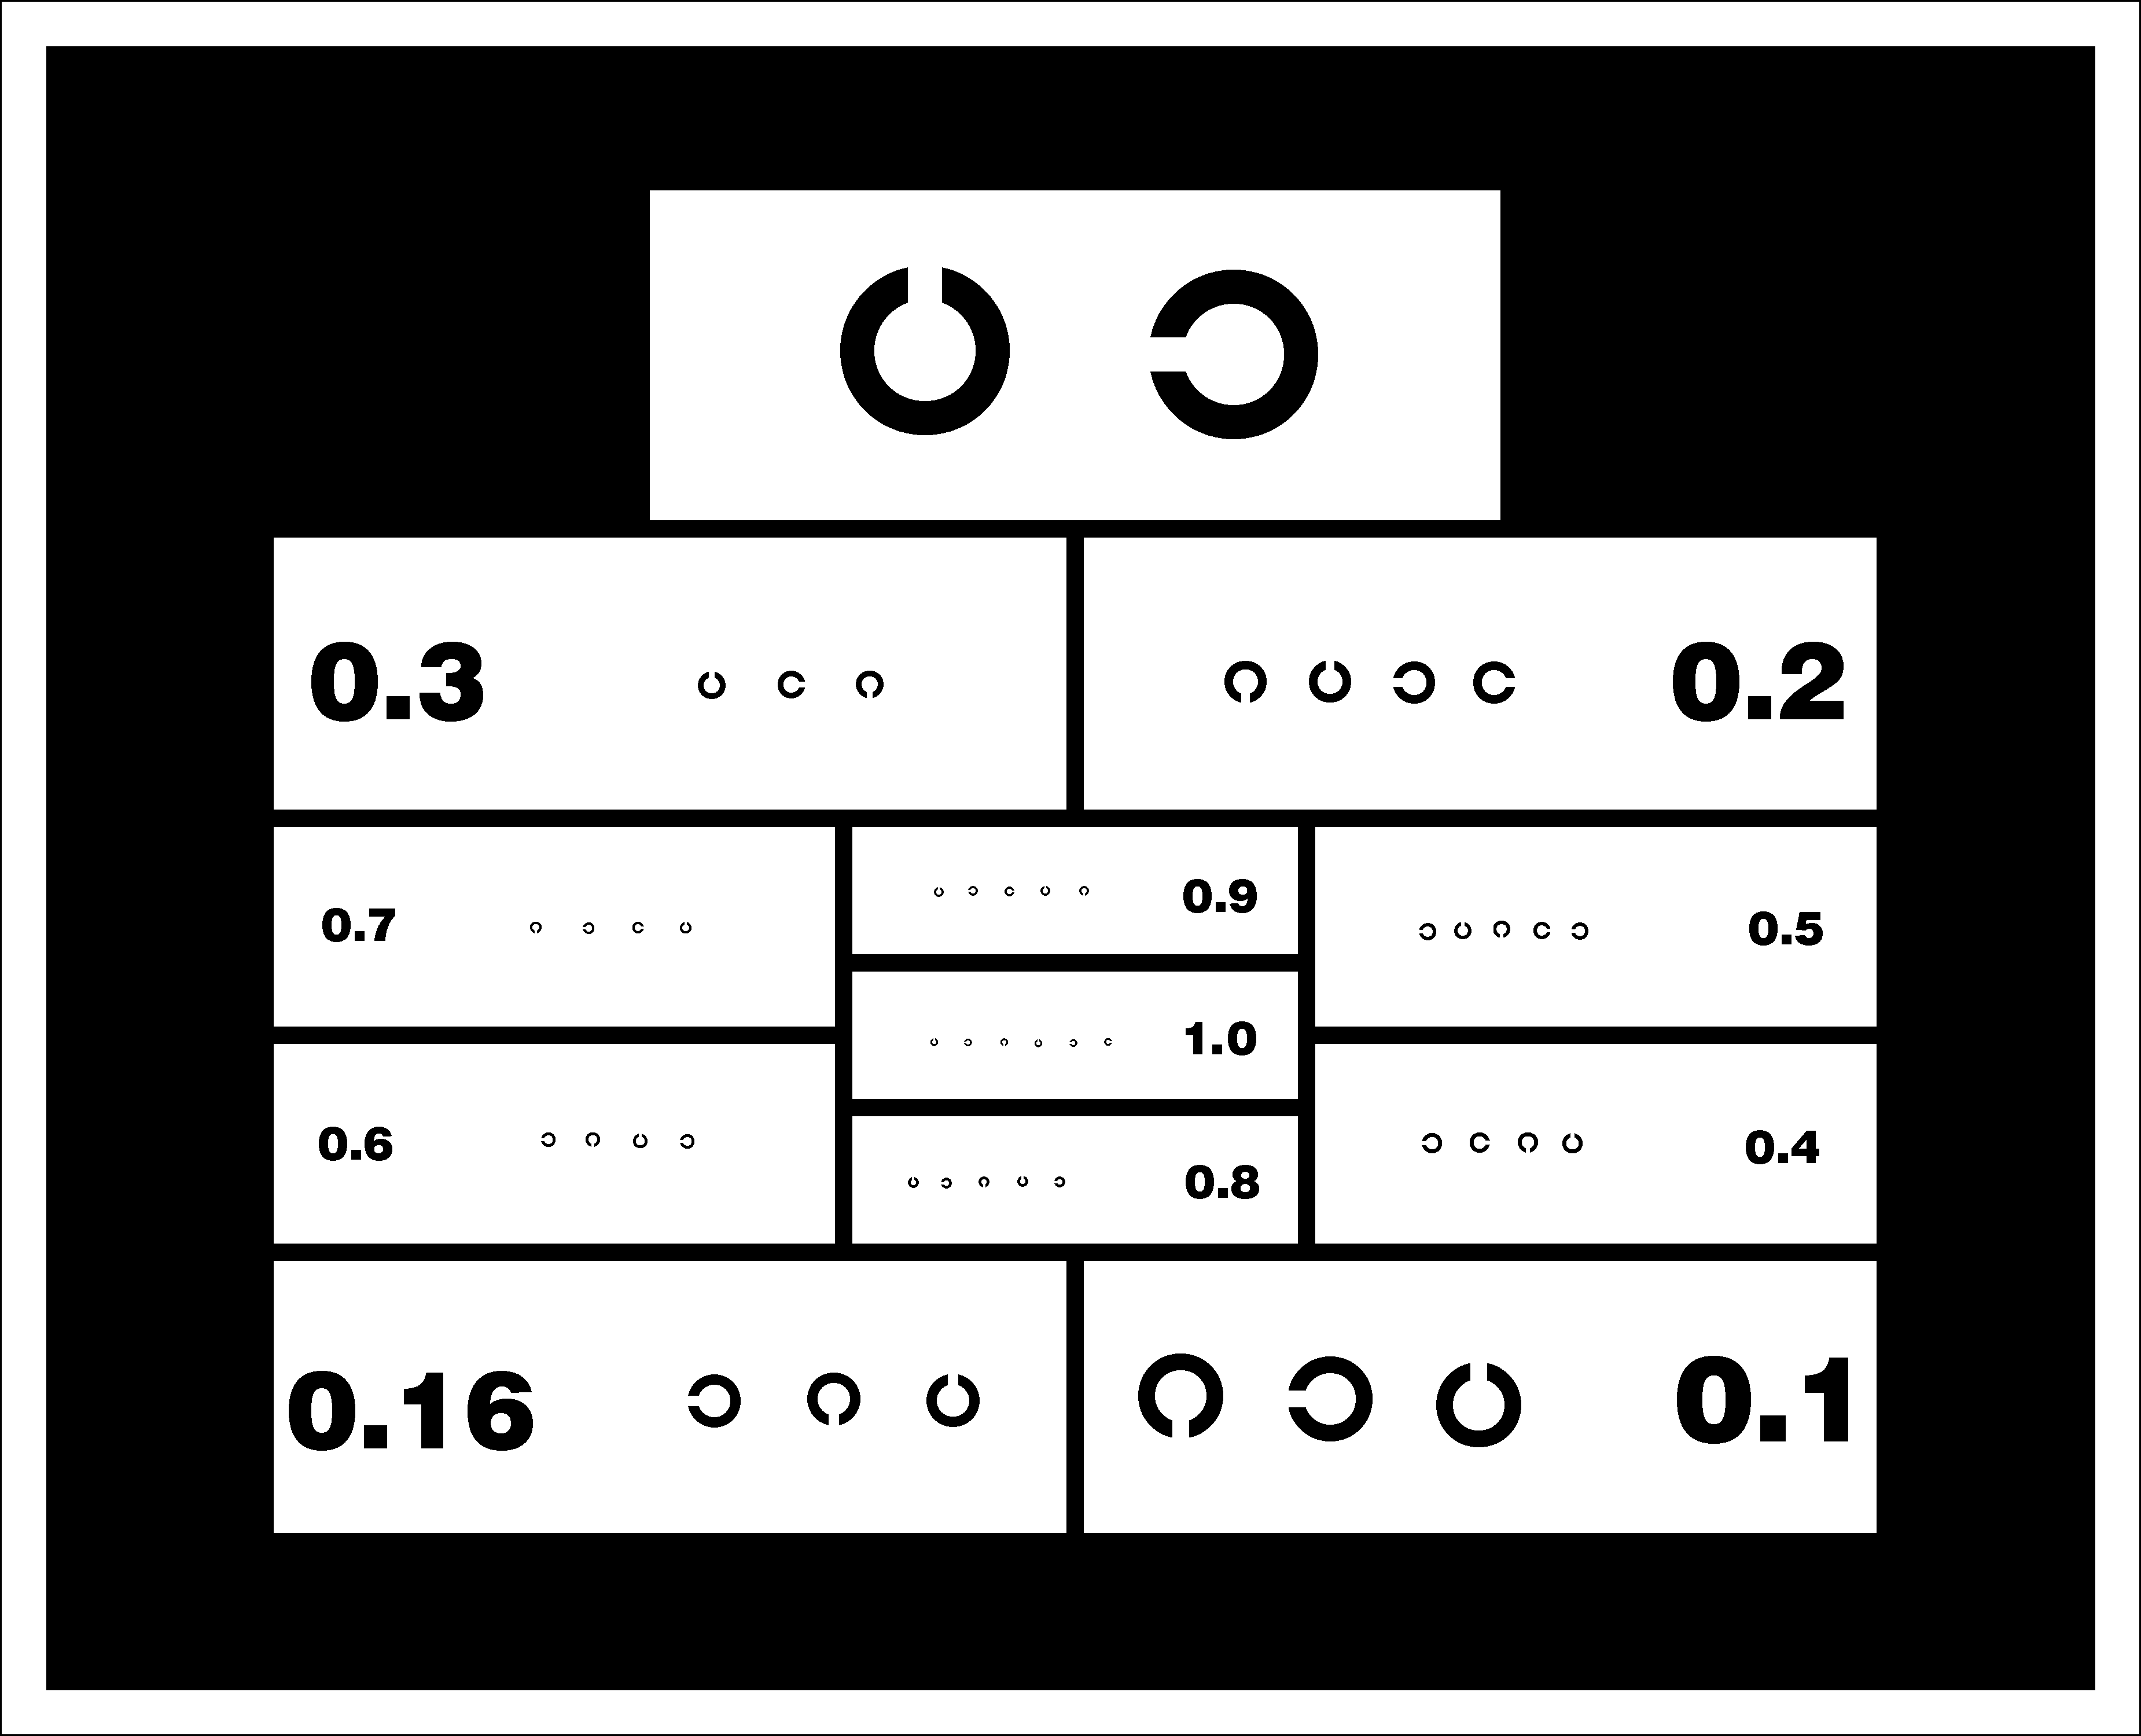
\includegraphics[scale=2]{Test_Obj_eye_control3.png}
        \caption{}
    \end{subfigure}
    \caption{ Тест-объекты для контроля остроты зрения.}
    \label{fig:TestObjEC}
\end{figure}

\section{Постановка задачи}
\textit{В этом пункте дописать мини-ТЗ, описать требования к оборудованию, П.О. и по пунктам описать необходимость интерфейсов, габариты, температурный режим и т.д.. Добавить описание конструкции с чертежами.}

Система автоматизации должна управлять устройством, общие принципы которого описаны выше, так чтобы выполнение всех необходимых функций, так же описанных выше, было простым, удобным, быстрым, эффективным как для врача(далее администратора), так и пациента(далее клиента).

\begin{figure}[ht]
	\centering
     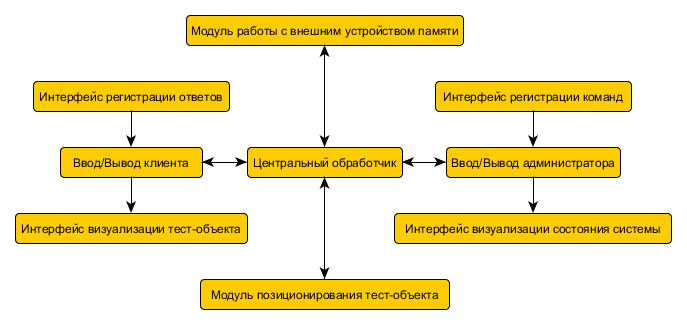
\includegraphics[scale=0.7]{function_shcem_of_sys_graf.jpg}
	\caption{Функциональная структура устройства.}
	\label{fig:graf:FunShcSys}
\end{figure}

 На блок-схеме(см.рис.\ref{fig:graf:FunShcSys}) показана функциональная структура устройства. Центральный обработчик - основной блок, выполняет  задачи транзакций между модулями, статистическую обработку данных, расчет графической оболочки, управление периферией и работу с внешним запоминающим устройством.

\begin{sidewaysfigure}

\centerline{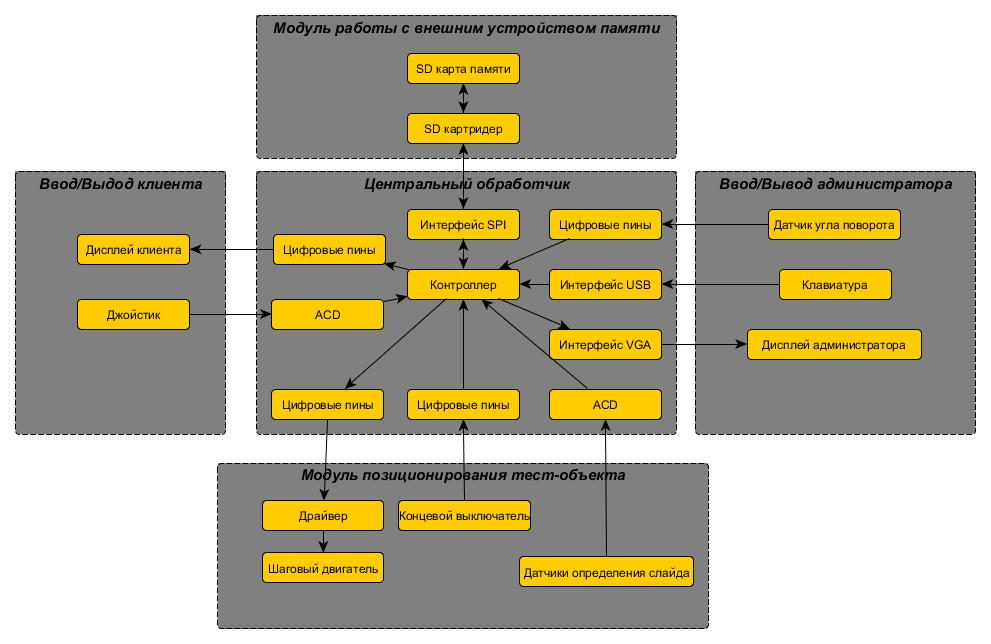
\epsfig{file=./images/apparats_shcem_of_sys_graf.jpg, scale=0.7}}

\caption{Аппаратная структура устройства.}
\label{fig:graf:AppShcSys}

\label{label_this_fig}

\end{sidewaysfigure}
На блок-схеме(см.рис.\ref{fig:graf:AppShcSys}) показана аппаратная структура устройства.
Далее в следующих главах мы выберем компонентную базу,подробно изучим элементы аппаратной структуры устройства, спроектируем электрическую разводку и перейдем к операционной системе.